\subsection*{Classe Subtree}
\label{sec:subtree-class}

\begin{figure}[H]
    \centering
    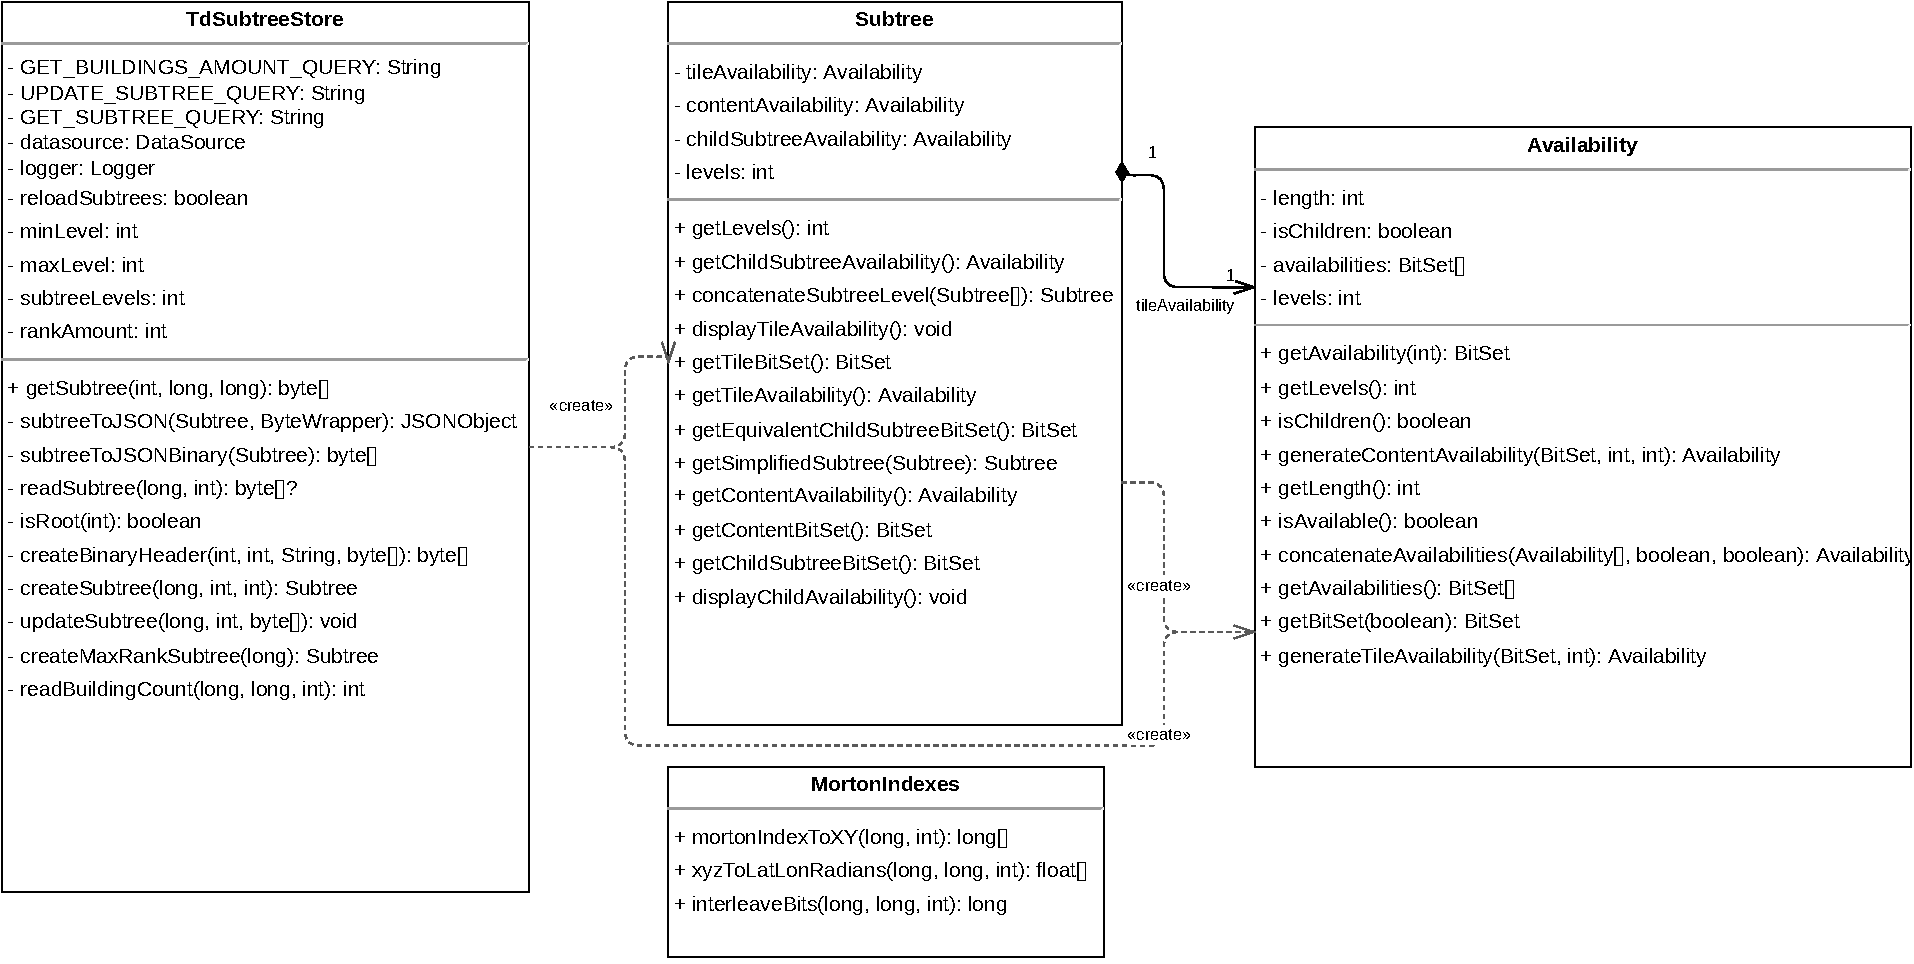
\includegraphics[width=1\textwidth]{assets/figures/subtree-classes.drawio.pdf}
    \caption{Classes utilisées pour la création d'une hiérarchie de Subtrees}
    \label{fig:subtree-classes}
\end{figure}

La première classe écrite dans le but de gérer les Subtrees est la classe \texttt{Subtree}. Un objet de cette classe comporte tout les éléments nécessaires pour la gestion d'un Subtree. Il contient un objet \texttt{Availability} pour chaque type de disponibilité (tuile, contenu, enfants) ainsi que le nombre de levels contenu. La classe offre aussi tous les getters utiles pour accéder aux informations importantes. Elle fournit aussi une fonction statique de concaténation de 4 Subtrees en un d'ordre supérieur. Cette fonction sera utilisée pour la création de l'arbre de Subtrees. Finalement, elle offre deux fonction de debug pour afficher les \textit{Tile Availability} et le \textit{Child Availability} dans la console.

\subsection*{Classe Availability}
\label{sec:availability-class}

La classe Availability est celle qui se chargera de stocker les listes de disponibilités. Pour cela, elle utilise un \textit{BitSet} par soucis d'optimisation. Tout comme la classe Subtree, elle offre une fonction de concaténation de 4 \textit{Availability} en une seule. De plus, elle propose deux fonctions pour générer un Availability complet à partir d'un BitSet représentant le dernier level du Subtree.

\subsection*{Classe TdSubtreeStore}
\label{sec:tdsubtreestore-class}

Cette classe est celle qui orchestrera la création et la distribution des Subtrees. Ce processus suit le diagramme suivant :

\begin{figure}[H]
    \centering
    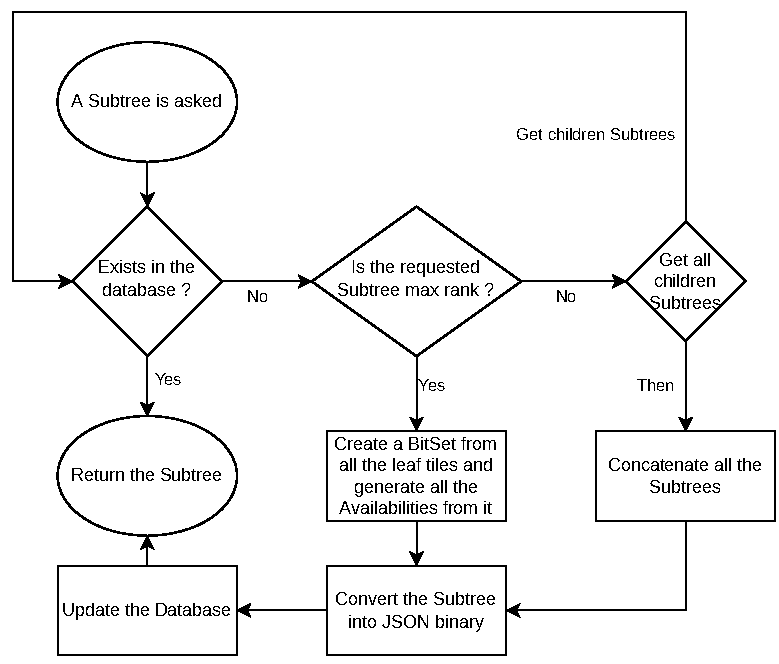
\includegraphics[width=1\textwidth]{assets/figures/simple-flowchart.drawio.pdf}
    \caption{Classes utilisées pour la création d'une hiérarchie de Subtrees}
    \label{fig:ssimple-flowchart}
\end{figure}

